\section{Sprint 3}
Der Fokus des dritten Sprints liegt bei der Verbesserung der Benutzererfahrung.
Das Ziel ist es, dass die Anwendung danach für die täglichen Arbeiten der Entwickler eingesetzt werden kann.
Dazu sind die folgende beiden Stories geplant:
\begin{itemize}
   \item DlmsQuickAccess soll mehrere, unterschiedliche Stromzählermodelle unterstützen.
   \item Ein Lese- oder Schreibbefehl soll nur dann abgesetzt werden können, wenn dieser laut Object Model vom jeweiligen Objekt unterstützt wird.
\end{itemize}

% Die grösste Lücke besteht aktuell noch darin, dass es nicht möglich ist, zwischen verschiedenen Zähler-Modellen zu wechseln.
% Es ist lediglich möglich mit dem Referenzprodukt "Ref\_MMI3" zu kommunizieren.



\subsection{Unterstützung für unterschiedliche Stromzählermodelle}
\dq DlmsQuickAccess soll mehrere, unterschiedliche Stromzählermodelle unterstützen.\dq
\subsubsection{Ziel}
Im Abschnitt \ref{picasso} wurde erwähnt, dass die Picasso Plattform über mehrere Referenzprodukte verfügt.
Drei dieser Referenzprodukte, namentlich \textit{Ref\_IMS1}, \textit{Ref\_NMS2} und \textit{Ref\_MMI3}, werden für die Arbeiten an der Plattform täglich verwendet.
Das Ziel dieser Story ist es, dass DlmsQuickAccess mit allen drei kommunizieren kann.
Im Bezug auf die \ac{DLMS} Kommunikation unterscheiden sich diese in zwei Dingen.
Zum Einen werden verschiedene Kommunikationskanäle verwendet. 
Während bei \textit{Ref\_MMI3} seriell mittels optischem Auslesekopf kommuniziert wird, wird bei \textit{Ref\_NMS2} eine \ac{TLS} Verbindung aufgebaut.
Der zweite Unterschied ist das Object Model, welches je nach Produkt andere Objekte enthält.
Damit die Story als erledigt betrachtet werden kann, sind noch folgende Punkte zu beachten:
\begin{itemize}
   \item Die Konfiguration eines Produkts soll in einer Datei abgespeichert werden. Wird diese Datei angeklickt, so soll sich der DlmsQuickAccess mit der darin enthaltenen Konfiguration gestartet werden.
   \item Wird der DlmsQuickAccess ohne Produktkonfiguration gestartet, so soll eine Auswahl von zuvor geöffneten Konfigurationen angezeigt werden.
   \item Den Benutzern sollen funktionierende Konfigurationen für die drei genannten Referenzprodukte bereitgestellt werden.
   \item Auf der Landis+Gyr internen Wiki soll ein Artikel geschrieben werden, welche Auskunft über DlmsQuickAccess und die Konfigurationsdateien gibt.
\end{itemize}

\subsubsection{Vorgehen und Schwierigkeiten}\label{s3configvorgehen}
Wie in Abschnitt \ref{firstRelease} beschrieben, funktioniert die Anwendungen bisher nur mit dem Produkt \textit{Ref\_MMI3}.
Dies hat damit zu tun, das einige produktspezifische Dateien bisher mit der Anwendung ausgeliefert werden und nicht anpassbar sind.
Eine dieser Dateien ist das Object Model als XML. 
Dieses wird, wie im Abschnitt \ref{visualizeOM} erläutert, für die Visualisierung der einzelnen Objekte benötigt und unterscheidet sich von Produkt zu Produkt.
Der Kommunikationscode des \ac{ATS} benötigt ein File mit der Konfiguration des Kommunikationskanals, dieses wird \textit{SetupHW} genannt.
Das \textit{SetupHW} File referenziert eine Adressliste, welche relativ zu ihm abgelegt sein muss.
Da alle Produkte der Picasso Plattform mit dem \ac{ATS} getestet werden, sind alle benötigten Konfigurationsdateien bereits vorhanden.
Für die Referenzprodukte sind sie im Repository der Testscripts abgelegt.

Der bisherige Ansatz, die Dateien als Teil der Anwendung an die Benutzer auszulieferen, hat nur einen Vorteil.
Die Anwendung kann nach der Installation direkt verwendet werden.
Es werden keine weiteren Dateien oder manuelle Konfigurationen benötigt.
Der Nachteil, dass bei jeder Änderung an der Konfiguration eine neue Version der Applikation erstellt und veröffentlicht werden muss, überwiegt diesen jedoch, da beispielsweise das Object Model regelmässig angepasst wird.
Ein weiterer Nachteil ist, dass um mit einer älteren Version der Firmware kommunizieren zu können auch eine ältere Version des DlmsQuickAccess installiert werden müsste.

Der zu ersetzende \ac{DMT2} wird über Textfiles konfiguriert.
Um das Produkt zu wechseln, muss jeweils das entsprechende Textfile importiert werden.
Diese Textfiles sind im Repository der Firmware abgelegt und somit versioniert.
Die importierte Konfiguration bleibt jeweils sitzungsübergreifend erhalten.
Dies wurde von den Nutzer als unpraktisch gemeldet, da beim Start der Anwendung nicht ersichtlich ist, welche Konfiguration aktiv ist.

Da auch andere Konfigurationen, wie beispielsweise jene des Debuggers oder des FlashTools im Repository des Firmwarecodes abgelegt sind, soll auch jene des DlmsQuickAccess dort verwaltet werden.
Die benötigten Object Models sind ebenfalls bereits Teil des Repository.
Im Picasso Projekt ist \ac{YAML} die bevorzugte Sprache für Konfigurationsdateien.

Basierend auf diesen Überlegungen und Hintergründen wurde folgende Lösung entwickelt:

Für jedes Produkt wird eine Konfigurationsdatei erstellt.
Der Name dieser endet auf .dlmsquickaccess.
Ihre Struktur sieht wie folgt aus:
\begin{verbatim}
Name: Ref_NMS2
ObjectModel: ObjectModel\\ObjectModel_Ref_NMS2.xml
SetupHW: SetupHW1Ref_NMS2.xml
\end{verbatim}
Die Konfigurationsdateien der Referenzprodukte werden im Repository der Firmware abgelegt.
Das \textit{SetupHW} File wird vom Repository der Testscripts in jenes der Firmware kopiert.
Die Applikation wird so angepasst, dass sie mittels Klick auf eine Konfigurationsdatei gestartet werden kann.
Dabei wird jeweils direkt die entsprechende Konfiguration angewendet.

Diese Lösung ermöglicht eine flexible Konfiguration der Produkte.
Dass das \textit{SetupHW} File aus dem Testscript Repository kopiert und somit manuell gepflegt werden muss ist nicht optimal, bietet jedoch den Vorteil, dass keine direkte Abhängigkeit zu weiteren Repositories besteht.

Wie beschrieben, wurde die Anwendung so angepasst, dass sie direkt über eine .dlmsquickaccess Datei gestartet werden kann.
Für den Fall, dass sie ohne eine solche gestartet wird, wurde ein neues Fenster implementiert.
Dieses listet alle bisher geöffneten Konfigurationen auf, welche direkt gestartet werden können.
Des weiteren war es geplant, dass mittels File-Picker eine Konfiguration gesucht und geöffnet werden kann.
Dies konnte jedoch nicht umgesetzt werden.
Die dazu benötigte Komponente von WinUI3, \textit{FileOpenPicker}, funktionierte zu jenem Zeitpunkt nur fehlerhaft\footnote{https://github.com/microsoft/WindowsAppSDK/issues/1188}.


Die neuen Konfigurationsfiles ermöglichen das einfache Wechseln zwischen verschiedenen Produkten.
Als versucht wurde, mit einem \textit{Ref\_NMS2} Zähler zu kommunizieren, führte dies regelmässig zu Fehlern.
Wurden die Integrationstest mit einem \textit{Ref\_NMS2} Gerät ausgeführte, so schlug jeweils jeder zweite Test fehl.
Dies wurde von der \ac{TLS} Kommunikation verursacht, welche nach dem Kommunizieren nicht richtig beendet wurde.
Für die Tests konnte das Schliessen der Verbindung jeweils in einer \textit{TestCleanup} Funktion aufgerufen werden.
In der Applikation konnte der \textit{OnClose} Event der \textit{Window} Klasse abonniert werden, um die Verbindung beim Schliessen des Fensters zu beenden.
Dieser Event wird jedoch nur dann ausgelöst, wenn die Applikation vom User geschlossen wird und nicht wenn sie abstürzt.


An Ende des Sprints konnte diese Story noch nicht geschlossen werden, da sich die Konfigurationsdateien noch nicht im Repository der Firmware befanden.
Der entsprechende Commit wartete noch auf ein Review.
Da dies direkt zu Beginn des nächsten Sprints erfolgte und alle anderen Arbeiten in diesem Sprint erledigt werden konnten, wird diese Story im Text zum Sprint 4 (\ref{sprint4}) nicht erwähnt.


\subsection{Deaktivieren von Lese- und Schreibknöpfen}
Das Feld \textit{Access Rights} im Object Model gibt an, ob ein Attribut gelesen und/oder geschrieben werden kann.
Für diese Story wurde die Benutzerschnittstelle so angepasst, dass die Lese- und Schreibknöpfe nur bei jenen Attributen aktiv sind, bei denen die entsprechende Operation möglich ist.
In Abbildung \ref{fig:logicalNameAttribute} ist ein \textit{logical\_name} Attribut gezeigt, welches nur gelesen und nicht geschrieben werden kann.

\begin{figure}[H]
   \centering
   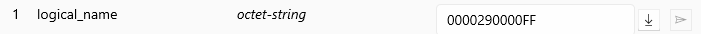
\includegraphics[width=1.0\textwidth]{gfx/logicalNameAttribute.png}
   \caption{
      Ausschnitt aus DlmsQuickAccess welcher ein einzelnes Attribut zeigt, welches gelesen, jedoch nicht geschrieben werden kann.
      }
      \label{fig:logicalNameAttribute}
   \end{figure}